%!TEX output_directory = temp
\documentclass[letterpaper, 12pt]{amsart}
	%%%%%%%%%%%%%%%%%%%%%%%%%%%%%%%%%%%%%%%%%%%%%%%%%%%%%%%%%%%%%%%%%%%%%%%%%%%%%%
	%%%%%%%%%%%%%%%%%%%%%%%%%%%% boilerplate packages %%%%%%%%%%%%%%%%%%%%%%%%%%%%
	\usepackage{amsmath,amssymb,amsthm}
	\usepackage[mathscr]{euscript}
	\usepackage{enumerate}
	\usepackage{graphicx}
	\usepackage{mathrsfs}
	\usepackage{color}
	\usepackage{hyperref}
	\usepackage{verbatim}
	\usepackage{stmaryrd}
	\usepackage[margin=1.25in]{geometry}

	\raggedbottom

	%%%%%%%%%%%%%%%%%%%%%%%%%%%%%%%%%%%%%%%%%%%%%%%%%%%%%%%%%%%%%%%%%%%%%%%%%%%%%%
	%%%%%%%%%%%%%%%%%%%%%%%%%%%%% rename the abstract %%%%%%%%%%%%%%%%%%%%%%%%%%%%
	% \renewcommand{\abstractname}{Introduction}

	%%%%%%%%%%%%%%%%%%%%%%%%%%%%%%%%%%%%%%%%%%%%%%%%%%%%%%%%%%%%%%%%%%%%%%%%%%%%%%
	%%%%%%%%%%%%%%%%%%%%%%%%%%%%%%%%%%%%% sets %%%%%%%%%%%%%%%%%%%%%%%%%%%%%%%%%%%
		%% sets 
		\DeclareMathOperator{\N}{\mathbb{N}}
		\DeclareMathOperator{\Z}{\mathbb{Z}}
		\DeclareMathOperator{\Zp}{\mathbb{Z}^{+}}
		\DeclareMathOperator{\Q}{\mathbb{Q}}
		\DeclareMathOperator{\Qp}{\mathbb{Q}^{+}}
		\DeclareMathOperator{\Qc}{\mathbb{Q}^{c}}
		\DeclareMathOperator{\R}{\mathbb{R}}
		\DeclareMathOperator{\F}{\mathbb{F}}
		\DeclareMathOperator{\Rp}{\mathbb{R}^{+}}
		\DeclareMathOperator{\C}{\mathbb{C}}
		\DeclareMathOperator{\Cnon}{\mathbb{C}^{\times}}
		%% powerset of a set
		\DeclareMathOperator{\pset}{\mathcal{P}}
		%% set of continuous functions in a certain variable
		\DeclareMathOperator{\cont}{\mathscr{C}}
		%% set of functions in a certain variable
		\DeclareMathOperator{\func}{\mathscr{F}}
		
	%%%%%%%%%%%%%%%%%%%%%%%%%%%%%%%%%%%%%%%%%%%%%%%%%%%%%%%%%%%%%%%%%%%%%%%%%%%%%%
	%%%%%%%%%%%%%%%%%%%%%%%%%%%%%%%% linear algebra %%%%%%%%%%%%%%%%%%%%%%%%%%%%%%
		%% linear span
		\DeclareMathOperator{\Ell}{\mathscr{L}}
		%% bold vectors with arrows, and bold matrices
		\newcommand{\bmat}[1]{{\mathbf{#1}}}
		\newcommand{\bvec}[1]{{\vec{\mathbf{#1}}}}
		%% independent vectors/matrices
		\DeclareMathOperator{\ind}{\perp\!\!\!\perp}
		%% order
		\DeclareMathOperator{\ord}{\text{ord}}

	%%%%%%%%%%%%%%%%%%%%%%%%%%%%%%%%%%%%%%%%%%%%%%%%%%%%%%%%%%%%%%%%%%%%%%%%%%%%%%
	%%%%%%%%%%%%%%%%%%%%%%%%%%% probability & statistics %%%%%%%%%%%%%%%%%%%%%%%%%
		%% probability, expectation, variance, etc.
		\renewcommand{\Pr}{\mathbb{P}}
		\DeclareMathOperator{\E}{\mathbb{E}}
		\DeclareMathOperator{\var}{\rm Var}
		\DeclareMathOperator{\sd}{\rm SD}
		\DeclareMathOperator{\cov}{\rm Cov}
		\DeclareMathOperator{\SE}{\rm SE}
		\DeclareMathOperator{\ssreg}{{\rm SS}_{{\rm Reg}}}
		\DeclareMathOperator{\ssr}{{\rm SS}_{{\rm Res}}}
		\DeclareMathOperator{\sst}{{\rm SS}_{{\rm Tot}}}

	%%%%%%%%%%%%%%%%%%%%%%%%%%%%%%%%%%%%%%%%%%%%%%%%%%%%%%%%%%%%%%%%%%%%%%%%%%%%%%
	%%%%%%%%%%%%%%%%%%%%%%%%%%%%%%%% congruences %%%%%%%%%%%%%%%%%%%%%%%%%%%%%%%%%
		\renewcommand{\mod}[1]{\ (\mathrm{mod}\ #1)}

	%%%%%%%%%%%%%%%%%%%%%%%%%%%%%%%%%%%%%%%%%%%%%%%%%%%%%%%%%%%%%%%%%%%%%%%%%%%%%%
	%%%%%%%%%%%%%%%%%%%%%%%%%%%%%% bracket notation %%%%%%%%%%%%%%%%%%%%%%%%%%%%%%
		% I first used this for principal ideals, that is why the abbreviation is pid
		\newcommand{\pid}[1]{\langle #1 \rangle}

	%%%%%%%%%%%%%%%%%%%%%%%%%%%%%%%%%%%%%%%%%%%%%%%%%%%%%%%%%%%%%%%%%%%%%%%%%%%%%%
	%%%%%%%%%%%%%%%%%%%%%%%%%%%%%%% fatdot notation %%%%%%%%%%%%%%%%%%%%%%%%%%%%%%
		\makeatletter
			\newcommand*\fatdot{\mathpalette\fatdot@{.5}}
			\newcommand*\fatdot@[2]{\mathbin{\vcenter{\hbox{\scalebox{#2}{$\m@th#1\bullet$}}}}}
		\makeatother

	%%%%%%%%%%%%%%%%%%%%%%%%%%%%%%%%%%%%%%%%%%%%%%%%%%%%%%%%%%%%%%%%%%%%%%%%%%%%%%
	%%%%%%%%%%%%%%%%%%%%%%%%%%%%%% use pretty letters %%%%%%%%%%%%%%%%%%%%%%%%%%%%
		\DeclareMathOperator{\ep}{\varepsilon}
		\DeclareMathOperator{\ph}{\varphi}

	%%%%%%%%%%%%%%%%%%%%%%%%%%%%%%%%%%%%%%%%%%%%%%%%%%%%%%%%%%%%%%%%%%%%%%%%%%%%%%
	%%%%%%%%%%%%%%%%%%%%%%%%%%% stolen from Jeske/Dugger %%%%%%%%%%%%%%%%%%%%%%%%%
	% Some theorem-like environments, all numbered together starting at 1
	% in each section.

	% The default \theoremstyle is bold headings and italic body text.
	\newtheorem{thm}{Theorem}[section]
	\newtheorem{defn}[thm]{Definition}
	\newtheorem{prop}[thm]{Proposition}
	\newtheorem{claim}[thm]{Claim}
	\newtheorem{cor}[thm]{Corollary}
	\newtheorem{lemma}[thm]{Lemma}

	\theoremstyle{definition}  % Bold headings and Roman body text.
	\newtheorem{example}[thm]{Example}
	\newtheorem{examples}[thm]{Examples}
	\newtheorem{exercise}[thm]{Exercise}
	\newtheorem{note}[thm]{Note}
	\newtheorem{remark}[thm]{Remark}
	\newtheorem{remarks}[thm]{Remarks}
	\newtheorem{discussion}[thm]{Discussion}

	\newcommand{\dfn}{\textbf} % Make defined words bold.
	\newcommand{\mdfn}[1]{\dfn{\mathversion{bold}#1}} % Even make math symbols bold

	% Various commands that are useful.  Please add your own.

	\DeclareMathOperator{\Arg}{Arg}
	\DeclareMathOperator{\re}{Re}
	\DeclareMathOperator{\im}{Im}
	\DeclareMathOperator{\Log}{Log}
	\DeclareMathOperator{\Span}{Span}

	\newcommand{\iso}{\cong}						% isometric/congruent
	\newcommand{\ra}{\rightarrow}                   % right arrow
	\newcommand{\Ra}{\Rightarrow}                   % right implies
	\newcommand{\lra}{\longrightarrow}              % long right arrow
	\newcommand{\la}{\leftarrow}                    % left arrow
	\newcommand{\La}{\Leftarrow}                    % left implies
	\newcommand{\lla}{\longleftarrow}               % long left arrow
	\newcommand{\llra}[1]{\stackrel{#1}{\lra}}      % labeled long right arrow
	\newcommand{\we}{\llra{\sim}}                   % weak equivalence
	\newcommand{\cof}{\rightarrowtail}              % cofibration
	\newcommand{\fib}{\twoheadrightarrow}           % fibration
	\newcommand{\inc}{\hookrightarrow}              % inclusion
	\newcommand{\dbra}{\rightrightarrows}           % double arrow for equalizer diagrams
	\newcommand{\eqra}{\llra{\sim}}                 % equivalence/isomorphism

	% \newcommand{\blank}{\underbar{\ \ }}          % An underscore, as in (__)xV
	\newcommand{\blank}{-}                          % A hyphen, as in (-)xV
	\newcommand{\Id}{Id}                            % The identity functor
	\newcommand{\und}{\underline}
	\newcommand{\norm}[1]{\mid \!\!#1 \!\!\mid}             %\norm{x} gives |x|

	% These commands are for the period and comma in the lower right entry of
	% a diagram.  They put the punctuation 2 pts to the right, but make
	% TeX (and hence the diagram package) unaware of the extra width
	% of that entry.
	\newcommand{\period}    {{\makebox[0pt][l]{\hspace{2pt} .}}}
	\newcommand{\comma}     {{\makebox[0pt][l]{\hspace{2pt} ,}}}
	\newcommand{\semicolon} {{\makebox[0pt][l]{\hspace{2pt} ;}}}

	\newcommand{\Cech}{\v{C}ech}
	\newcommand{\scat}{\Delta}
	\newcommand{\assign}{\ra}
	\newcommand{\copr}{\,\amalg\,}
	\newcommand{\ovcat}{\downarrow}
	\newcommand{\pder}[2]{{\frac{\partial #1}{\partial #2}}}
	\newcommand{\del}{\nabla}
	\newcommand{\vectr}[1]{{\mbox{\boldmath $#1$}}}
	\newcommand{\uvectr}[1]{\vectr{\hat #1}}
	\newcommand{\ihat}{\uvectr \imath}
	\newcommand{\jhat}{\uvectr \jmath}
	\newcommand{\khat}{\uvectr k}
	\newcommand{\rhat}{\uvectr r}
	\newcommand{\thhat}{\uvectr \theta}
	\newcommand{\zhat}{\uvectr z}
	\newcommand{\rhohat}{\uvectr \rho}
	\newcommand{\phihat}{\uvectr \phi}
	\newcommand{\grad}{\vectr{\vec\nabla}}
	% \newcommand{\R}{\mathbb{R}}
	\newcommand{\vv}[1]{\vectr{v_{#1}}}
	\newcommand{\crad}{0.1}
	\newcommand{\lline}[1]{\overleftrightarrow{#1}}
	\DeclareMathOperator{\area}{area}
	\DeclareMathOperator{\vol}{vol}
	\newcommand{\ray}[1]{\overset{\rightarrow}{#1}}
	\newcommand{\sr}[2]{???}
	\newcommand{\iihat}{i}
	\newcommand{\jjhat}{j}
	\newcommand{\kkhat}{k}

	\renewcommand{\abstractname}{Comment}		
\begin{document}
	\title{Homework 4  -- Math 397 \\ \today}
	\author{Alex Thies \\ \href{mailto:athies@uoregon.edu}{\lowercase{athies$@$uoregon.edu}}}

	\maketitle

	\section*{Problem 2}
	This problem concerns ellipses, which are the solutions sets of equations of the form $$\frac{x^{2}}{a^{2}} + \frac{y^{2}}{b^{2}} = 1$$ where $a, b > 0$. 
	Assume $b \leq a$. 
	The eccentricity of the ellipse is defined by the formula $e = \sqrt{1 - (b/a)^{2}}$ and this always lies in $[0, 1)$. 
	The eccentricity of a circle is $0$, and when $e$ is close to $1$ the ellipses are long and thin.

		\subsection*{Part (a)}
		The points $F_{1} = (-ae, 0)$ and $F_{2} = (ae, 0)$ are called the \textbf{foci} of the ellipse. 
		Show that the distance $QF_{2}$ in the picture below is equal to $a$:
		\begin{figure}[h]
			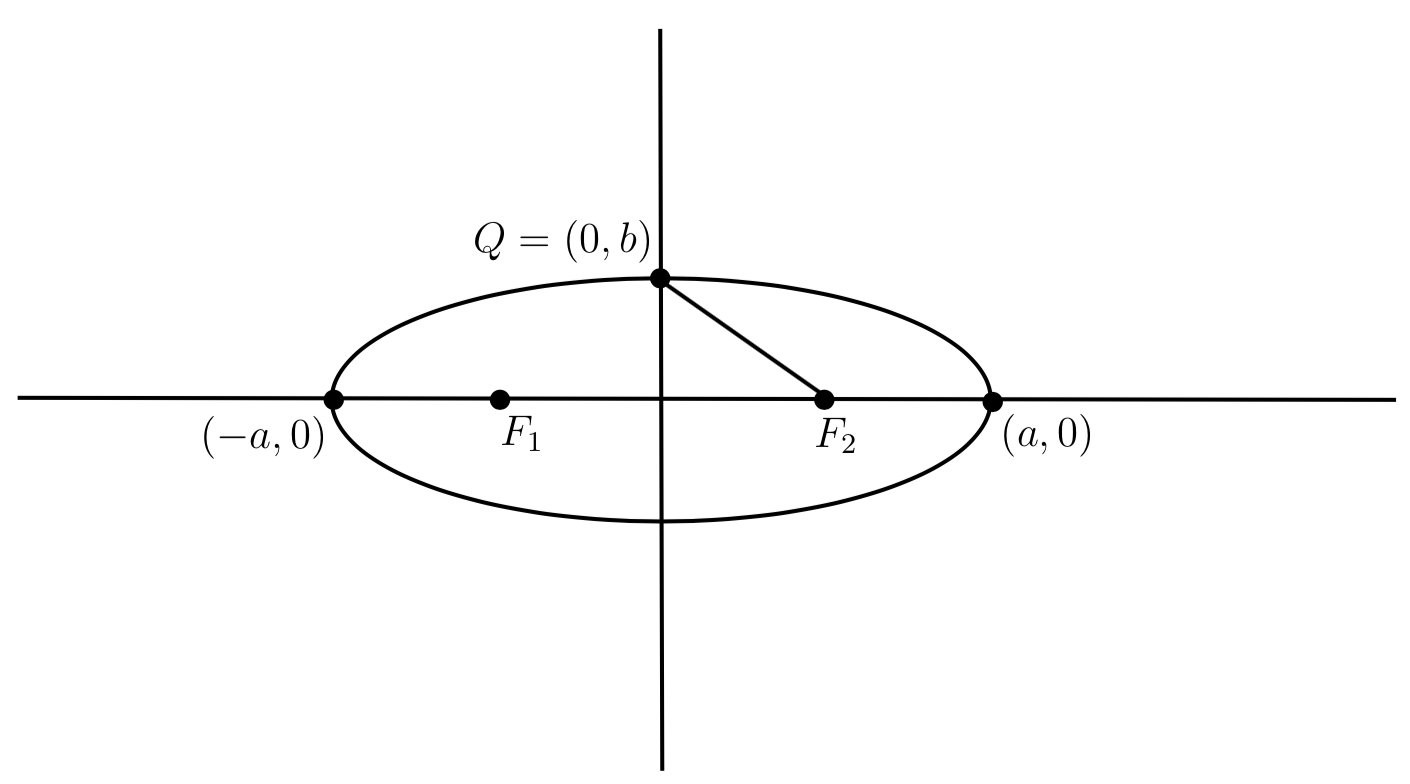
\includegraphics[width=0.5\textwidth]{images/ellipse.png}
			% \caption{An Ellipse}
			\label{ellipse}
		\end{figure}

		\begin{proof}[Solution]
		We compute the following:
			\begin{align*}
				d(Q,F_2) &= \sqrt{(ae - 0)^2 + (0 - b)^2}, \\
	            &= \sqrt{(ae)^2 + b^2}, \\
	            &= \sqrt{a^2 \left(1 - \tfrac{b^2}{a^2} \right) + b^2}, \\
	            &= \sqrt{a^2 - b^2 + b^2}, \\
	            &= \sqrt{a^2}, \\
	            &= |a|, \\
				&= a.
			\end{align*}
									
		\end{proof}
		% subsection part_a (end)

		\subsection*{Part (b)}
		Show that for points $P$ on the ellipse the distance $F_{1}P +PF_{2}$ is always equal to $2a$.
		[Hint: Let $P = (x, y)$. 
		Write down a formula for the total distance function $d(x, y) = d(P, F_{1}) + d(P, F_{2})$ in terms of $x, y, a, b$, and $e$. 
		Use the equation for the ellipse to eliminate all $y$ variables, and then use $a^{2}e^{2} = a^{2} − b^{2}$ to eliminate $b$. 
		The algebra is a little involved, but not terrible.]

		\begin{proof}[Solution]
		First let's make some tools for substitution.
		Solving the ellipse for $y$ yields $y^2 = b^2 - \tfrac{b^2}{a^2}x^{2}$; playing with the formula for eccentricity yields $a^2e^2 = a^2 - b^2$, further algebraic manipulation gives us $a^2e^2 = x^2 - x^2e^2$.
			We compute the following:
				\begin{align*}
				d(x,y) &= d(F_1,P) + d(P,F_2), \\
	            &= \sqrt{(x + ae)^2 + y^2} + \sqrt{(ae - x)^2 + (-y)^2}, \\
	            &= \sqrt{(x + ae)^2 + y^2} + \sqrt{(ae - x)^2 + y^2}, \\
				&= \sqrt{(x + ae)^2 + b^2 - \tfrac{b^2}{a^2}x^2} + \sqrt{(ae - x)^2 + b^2 - \tfrac{b^2}{a^2}x^{2}}, \\
				&= \sqrt{(x + ae)^2 + b^2 - \tfrac{b^2x^2}{a^2}} + \sqrt{(ae - x)^2 + b^2 - \tfrac{b^2x^2}{a^2}}, \\
	            &= \sqrt{(x + ae)^2 + a^2 - a^2e^2 - (x^2 - x^2e^2)} + \sqrt{(ae - x)^2 + a^2 - a^2e^2 - (x^2 - x^2e^2)}, \\
	            &= \sqrt{2xae + a^2 + x^2e^2} + \sqrt{a^2 + x^2e^2}, \\
	            &= \sqrt{(a + xe)^2} + \sqrt{(a - xe)^2}, \\
	            &= a + xe + a - xe, \\
	            &= 2a.
				\end{align*}
				
		\end{proof}
		% subsection part_b (end)

		\subsection*{Part (c)}
		For convenience just make $a = 1$ now. 
		Use Sage to draw a graph showing the circle of radius 1 and the ellipse with $a = 1$ and eccentricity $e = 0.75$, in different colors on the same graph. 
		(Hint: Implicit-Plot command, introduced on the last homework). 
		Include a picture of the graph as your solution for this part.

		\begin{proof}[Solution]
		See Figure \ref{circle1} for the unit circle and ellipse with eccentricity $e = 0.75$.
		\end{proof}
		% subsection part_c (end)

		\subsection*{Part (d)}
		Now vary the eccentricity and observe how the ellipse changes. 
		What is the smallest eccentricity where you can see a visible difference between the circle and ellipse? 
		Give one or two decimal places, and don’t feel like you have to find the \textit{absolute} smallest eccentricity -- an approximate answer is fine. 
		(You should choose an appropriate scale for this problem; if your circle and ellipse are a dot on the page you are not going to see anything).

		\begin{proof}[Solution]
			See Figure \ref{circle2} for the unit circle and ellipse with small eccentricity, $e = 0.12$.
			I plotted the circle, and an ellipse with eccentricity $e = 0$, and varied $e$ slightly until I could notice the slightest difference.
		\end{proof}
		% subsection part_d (end)

		\subsection*{Part (e)}
		Look up the eccentricities for the orbits of the planets, as well as Halley’s Comet. 
		Which orbits are you comfortable describing as ``nearly circular''?

		\begin{proof}[Solution]
			Observe Figure \ref{orbit} for the list of planetary eccentricities (looked up online), as well as for Halley's Comet.
			Based on work from the previous section, we would say that only Mercury, Pluto, and Halley's Comet do not have nearly circular orbits.

			\begin{figure}[h]
				\begin{tabular}{c|c}
					Celestial Body & Eccentricity \\
					\hline
					Mercury & 0.2488 \\
					Venus & 0.0068 \\
					Earth & 0.0167 \\
					Mars & 0.0340 \\
					Jupiter & 0.0484 \\
					Saturn & 0.0541 \\
					Neptune & 0.0086 \\
					Uranus & 0.0472 \\
					Pluto & 0.2488 \\
					Halley's Comet & 0.9671
				\end{tabular}
				\caption{Orbital Eccentricities of Local System Objects}
				\label{orbit}
			\end{figure}
		\end{proof}
		% subsection part_e (end)

		\subsection*{Part (f)}
		Points on the ellipse $\tfrac{x^{2}}{a^{2}} + \tfrac{y^{2}}{b^{2}} = 1$ can be described by $(x,y) = (r \cos\theta,r\sin\theta)$ where $r = r(\theta)$ is a function of $\theta$. 
		Plug into the equation of the ellipse, solve for $r$, and show that $$r = \frac{b}{\sqrt{1 - e^{2}\cos^{2}\theta}}.$$

		This is the equation for the ellipse in polar coordinates.

		\begin{proof}[Solution]
		We compute the following:
			\begin{align*}
				\frac{x^{2}}{a^{2}} + \frac{y^{2}}{b^{2}} &= 1, \\
				\frac{b^{2}}{a^{2}}(r \cos\theta)^{2} + (r\sin\theta)^{2} &= b^{2}, \\
				r^{2} \left( \frac{b^{2}}{a^{2}}\cos^{2}\theta + 1 - \cos^{2}\theta \right) &= b^{2}, \\
				r^{2} &= \frac{b^{2}}{\left( \tfrac{b^{2}}{a^{2}}\cos^{2}\theta + 1 - \cos^{2}\theta \right)}, \\
				&= \frac{b^{2}}{\left( 1 - \cos^{2}\theta + \tfrac{b^{2}}{a^{2}}\cos^{2}\theta \right)}, \\
			\end{align*}
			\begin{align*}
				&= \frac{b^{2}}{1 - \left( 1 - \tfrac{b^{2}}{a^{2}} \right)\cos^{2}\theta}, \\
				r &= \frac{b}{\sqrt{1 - e^{2}\cos^{2}\theta}}.
			\end{align*}
		Hence $r = \tfrac{b}{\sqrt{1 - e^{2}\cos^{2}\theta}}$, as we aimed to show.
		\end{proof}
		% subsection part_f (end)

		\subsection*{Part (g)}
		Sage can plot curves in polar coordinates. Try the command $$\verb|polar_plot(3/(1-0.7^2 * cos(s)^2)^(0.5),(s,0,2*pi))|$$ Then try the following modifications. 
		You don’t have to include graphs on your HW, but write a brief description of what is happening in each one.
			\begin{enumerate}[\hspace{5mm} (i)]
				\item Remove the square from the cos(s).
				\item Put the square back in, but change $\cos(s)$ to $\cos(7s)$.
				\item Change $\cos(s)$ to $\cos(15 + s)$.
				\item Change back to $\cos(s)$, but also change the $3$ in the numerator to $3s$.
				\item Same as previous part, but change the interval to $(0, 16\pi)$.
			\end{enumerate}

		\begin{proof}[Solution]
			See Figures \ref{figs1}, \ref{figs2}, and \ref{figs3} for the actual graphs.
			In (i), removing the square from the cosine makes the plot less eccentric, and moves the center.
			In (ii), returning the square and changing the argument makes the boundary of the circle change into a reflected cosine graph that has seven repititions over $0 \leq \theta \leq \pi$.
			In (iii), changing the argument again removes the weird boundary stuff, reintroduces some eccentricity, and seems to rotate the figure about the origin.
			In (iv) and (v), we get spirals with different rates.
		\end{proof}
		% subsection part_g (end)
	% section problem_2 (end)

	\begin{remark}
		I have some rough/messy work for problem 3 that is hand-written, but I lost track of how much of this assignment I had TeX-ed, and so I didn't have time to type everything up.
		I'm not including the rough work for two reasons: (1) its on my nightstand, and (2) I have a feeling it has several errors.
	\end{remark}

	\section*{Problem 3}
	The question concerns a spring-mass system with $m = k = 1$, so that the differential equation is $\ddot{x} + \gamma\dot{x} + x = 0$. 
	Assume that $\gamma^{2} < 4$, so that we have oscillatory solutions, and take the initial values $x(0) = 1$ and $x'(0) = 0$.

		\subsection*{Part (a)}
		Go through the steps of solving the differential equation and show that the solution has the form $$x(t) = e^{\frac{-\gamma}{2}t}\cdot\cos\left( \cos{(\omega t)} + \tfrac{\gamma}{2\omega}\cos{(\omega t)} \right)$$ where $\omega = \frac{\sqrt{4 - \gamma^{2}}}{2}$.
		% subsection part_a (end)

		\subsection*{Part (b)}
		Use Sage to plot the three solutions corresponding to $\gamma = 1$, $\gamma = 0.7$, and $\gamma = 0.5$ on one graph, in different colors.
		% subsection part_b (end)

		\subsection*{Part (c)}
		Let’s say that in real life the mass is stopped once the fluctuations from the equilibrium position are less than 0.01. 
		Use Sage to graphically estimate how long it takes for the mass to stop when $\gamma = 0.5$. 
		Give your answer to one decimal place (so something like 12.3, not just 12). 
		Explain (briefly) how you went about finding your answer.
		% subsection part_c (end)

		\subsection*{Part (d)}
		This time imagine two of our spring-mass systems side-by-side, one with $\gamma = 0.5$ and one with $\gamma = 0.7$. 
		These both have the same initial conditions of $x(0) = 1$ and $x'(0) = 0$, so in particular the masses are side-by-side at $t = 0$. 
		What is the next time that they are again side-by-side? 
		Use Sage to find out, giving your answer to 5 decimal places. 
		[Hint: Don’t do this graphically. 
		Have Sage solve an equation.]
		% subsection part_d (end)

		\subsection*{Part (e)}
		Sage can solve differential equations on its own. 
		Try the following commands:
			\begin{enumerate}[]
				\item \verb|f=function('f')(x)|

				\item \verb|desolve(diff(f,x,2)+0.5*diff(f,x,1)+f==0,dvar=f,ivar=x,ics=[0,1,0])|

				\item \verb|g=desolve(diff(f,x,2)+0.5*diff(f,x,1)+f==0,dvar=f,ivar=x,ics=[0,1,0])|

				\item \verb|plot(g(x),(x,0,20))|
			\end{enumerate}
		Sage can even solve the differential equation with an unspecified constant in it. 
		We will replace our $\gamma$ variable with `c' in Sage. 
		Try this:
			\begin{enumerate}[]
				\item \verb|c=var('c')|

				\item \verb|assume(c>0)|

				\item \verb|assume(c<2)|

				\item \verb|desolve(diff(f,x,2)+c*diff(f,x,1)+f==0,dvar=f,ivar=x,ics=[0,1,0])|

				\item \verb|assume(c>2)|

				\item \textbf{[The above command should have produced another error; think about why.]}

				\item \verb|forget(c<2)|

				\item \verb|assume(c>2)|

				\item \verb|desolve(diff(f,x,2)+c*diff(f,x,1)+f==0,dvar=f,ivar=x,ics=[0,1,0])|
			\end{enumerate}
		% subsection part_e (end)
	% section problem_3 (end)
	\newpage

	\section{Figures}
	\label{sec:figures}
		\begin{figure}[h]
			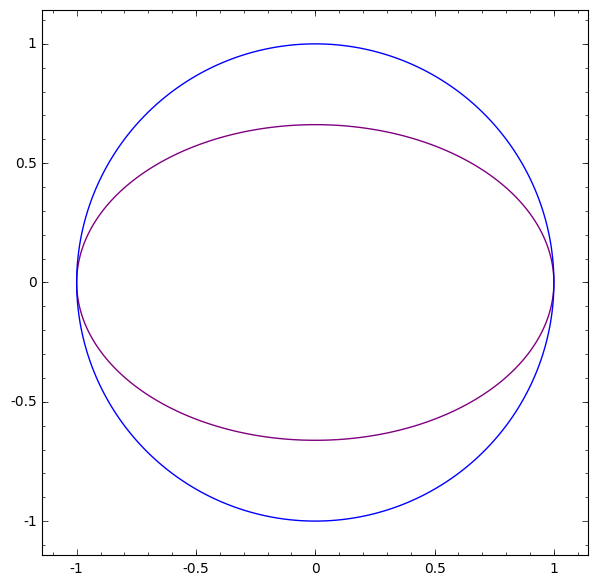
\includegraphics[width=0.55\textwidth]{images/2c.png}
			\caption{A unit circle, and an ellipse with $a=1$ and $e=0.75$.}
			\label{circle1}
		\end{figure}

		\begin{figure}[h]
			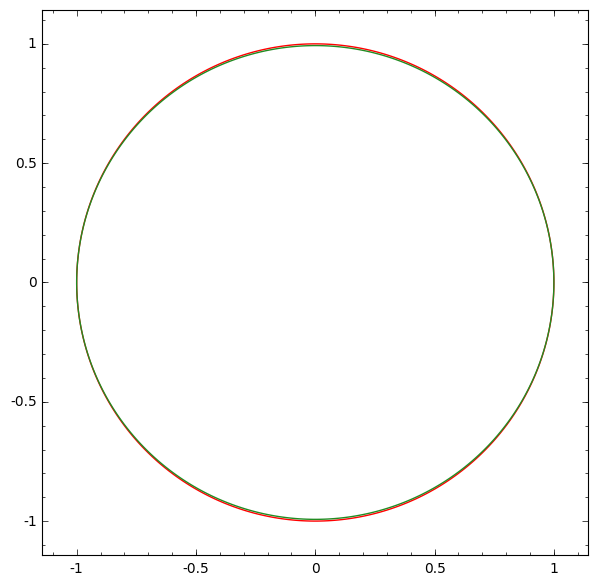
\includegraphics[width=0.55\textwidth]{images/2d.png}
			\caption{A unit circle, and an ellipse with $a=1$ and $e=0.12$.}
			\label{circle2}
		\end{figure}

		\begin{figure}[h]
			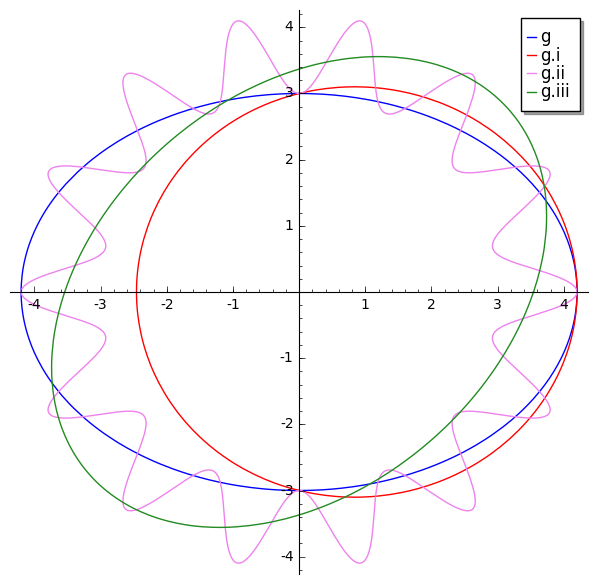
\includegraphics[width=0.55\textwidth]{images/2g_1.png}
			\caption{Steps 2.g.i - 2.g.iii}
			\label{figs1}
		\end{figure}

		\begin{figure}[h]
			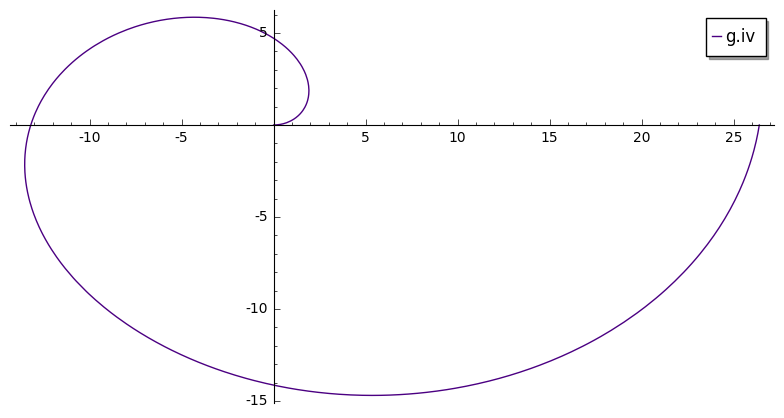
\includegraphics[width=0.55\textwidth]{images/2g_2.png}
			\caption{Step 2.g.iv}
			\label{figs2}
		\end{figure}

		\begin{figure}[h]
			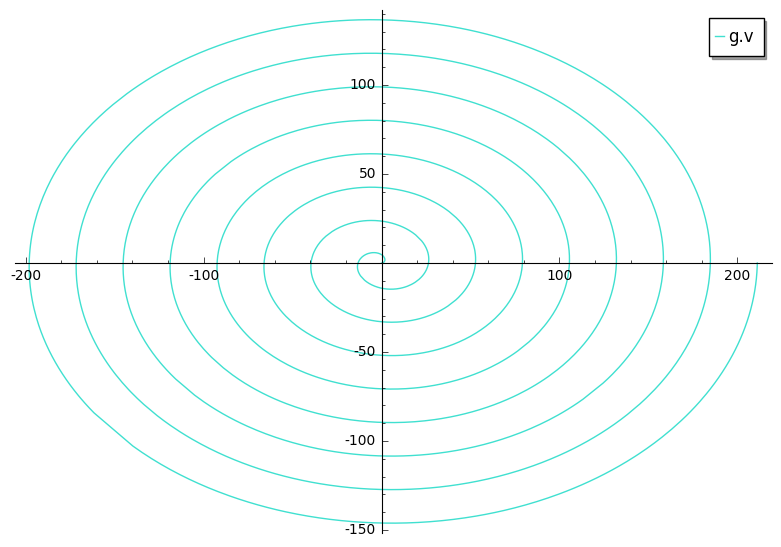
\includegraphics[width=0.5\textwidth]{images/2g_3.png}
			\caption{Step 2.g.v}
			\label{figs3}
		\end{figure}
	% section figures (end)
\end{document}